
%(BEGIN_QUESTION)
% Copyright 2008, Tony R. Kuphaldt, released under the Creative Commons Attribution License (v 1.0)
% This means you may do almost anything with this work of mine, so long as you give me proper credit

A technician brings a control power transformer into your repair shop for diagnosis.  It is a dual-voltage primary unit, and was used on the job site to step 480 volts down to 120 volts:

$$\includegraphics[width=15.5cm]{i03173x01.eps}$$

According to the person who did the field troubleshooting, the transformer is simply ``bad.''  As is typical, you were given no other information to help diagnose the precise fault.  Describe how you would test this transformer in your shop for the following faults, noting the transformer terminals you would connect your multimeter to and the type of meter measurement you would expect to see for each specified fault.

\vskip 10pt

\noindent
\underbar{First (left) primary winding failed open}
\begin{itemize}
\vskip 5pt
\item{} Meter connected between:
\vskip 5pt
\item{} Measurement expected for this type of fault:

\end{itemize}
\vskip 30pt

\noindent
\underbar{Second (right) primary winding failed open}

\vskip 5pt
\begin{itemize}
\item{} Meter connected between:
\vskip 5pt
\item{} Measurement expected for this type of fault:
\end{itemize}

\vskip 30pt

\noindent
\underbar{First (left) primary winding shorted to iron core}

\vskip 5pt
\begin{itemize}
\item{} Meter connected between:
\vskip 5pt
\item{} Measurement expected for this type of fault:
\end{itemize}

\vskip 30pt

\noindent
\underbar{Secondary winding shorted to iron core}

\vskip 5pt
\begin{itemize}
\item{} Meter connected between:
\vskip 5pt
\item{} Measurement expected for this type of fault:
\end{itemize}

\vfil 


\underbar{file i03173}
\eject
%(END_QUESTION)





%(BEGIN_ANSWER)

This is a graded question -- no answers or hints given!

%(END_ANSWER)





%(BEGIN_NOTES)

\noindent
\underbar{First (left) primary winding failed open}

\vskip 5pt
\item{} Meter connected between: {\it H1 and H2}
\vskip 5pt
\item{} Measurement expected for this type of fault: {\it Infinite resistance}

\vskip 30pt

\noindent
\underbar{Second (right) primary winding failed open}

\vskip 5pt
\item{} Meter connected between: {\it H3 and H4}
\vskip 5pt
\item{} Measurement expected for this type of fault: {\it Infinite resistance}

\vskip 30pt

\noindent
\underbar{First (left) primary winding shorted to iron core}

\vskip 5pt
\item{} Meter connected between: {\it Either H1 or H2, and metal frame/core of transformer}
\vskip 5pt
\item{} Measurement expected for this type of fault: {\it Low resistance}

\vskip 30pt

\noindent
\underbar{Secondary winding shorted to iron core}

\vskip 5pt
\item{} Meter connected between: {\it Either X1 or X2, and metal frame/core of transformer}
\vskip 5pt
\item{} Measurement expected for this type of fault: {\it Low resistance}

\vskip 30pt

Keep in mind that a healthy transformer winding should exhibit very little resistance end-to-end (from one terminal to another), but infinite resistance between either of its terminals and the metal frame (iron core).

\vskip 10pt

An even better piece of test equipment than a multimeter for the last two tests would be an {\it insulation tester}, often referred to by the common brand-name {\it Megger}.  This instrument uses relatively high voltage to check for the presence of high-resistance continuity, such as what happens when electrical insulation begins to break down.

%INDEX% Troubleshooting review: electric circuits

%(END_NOTES)


